% 2001 年上海卷理科第 19 题：正方体与动点
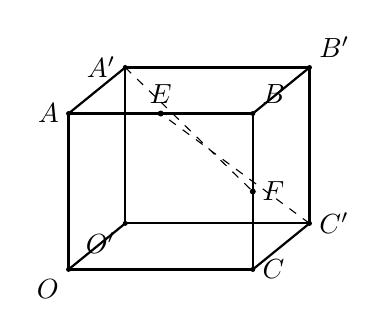
\begin{tikzpicture}[>=stealth, scale=0.9]
  \coordinate (O) at (0,0);
  \coordinate (A) at (0,2.2);
  \coordinate (B) at (2.6,2.2);
  \coordinate (C) at (2.6,0);
  \coordinate (O1) at (0.8,0.65);
  \coordinate (A1) at (0.8,2.85);
  \coordinate (B1) at (3.4,2.85);
  \coordinate (C1) at (3.4,0.65);
  \coordinate (E) at (1.3,2.2);
  \coordinate (F) at (2.6,1.1);

  \draw[thick] (O)--(A)--(B)--(C)--cycle;
  \draw[thick] (O1)--(A1)--(B1)--(C1)--cycle;
  \draw[thick] (O)--(O1) (A)--(A1) (B)--(B1) (C)--(C1);
  \draw[dashed] (A1)--(F) (C1)--(E);
  \fill (E) circle (1.2pt) node[above] {$E$};
  \fill (F) circle (1.2pt) node[right] {$F$};
  \fill (O) circle (1pt) node[below left] {$O$};
  \fill (A) circle (1pt) node[left] {$A$};
  \fill (B) circle (1pt) node[above right] {$B$};
  \fill (C) circle (1pt) node[right] {$C$};
  \fill (O1) circle (1pt) node[below left] {$O'$};
  \fill (A1) circle (1pt) node[left] {$A'$};
  \fill (B1) circle (1pt) node[above right] {$B'$};
  \fill (C1) circle (1pt) node[right] {$C'$};
\end{tikzpicture}
